\documentclass[twoside]{article}
\usepackage{styles}
% Imported Packages ==================
\usepackage{float}
\usepackage{xepersian}
\usepackage{fontspec}
\usepackage{amsmath}
\usepackage{amsfonts}
\usepackage{multirow}

% Font Settings ======================

\settextfont[Path = ./fonts/fa/, BoldFont={HMXKayhanBd}]{HMXKayhan}
\setlatintextfont[Path = ./fonts/latin/]{LinLibertine}
% Graphic Settings ===================
\usepackage{graphicx}
\graphicspath {{./images/} }
\DeclareGraphicsExtensions{.png,.jpg,.jpeg}

% Command Definements ================
\newcommand{\StudentID}{400105014}
\newcommand{\نام}{محمدعرفان سلیما}
\newcommand{\گروه}{2}
\newcommand{\CompileDate}{\today}
% ====================================

\begin{document}
% === DO NOT MAKE ANY CHANGES HERE ===
\maketitlebox
\section*{بخش تئوری}
من \نام{} به شماره دانشجویی \StudentID{} از اعضای گروه \گروه{} هستم و این پروژه آخرین بار در تاریخ \CompileDate{}
توسط موتور پردازشی \XeLaTeX تفسیر شده است.

% ====================================
\subsection*{سوال 1}
 با فرض اینکه x جزو مجموعه  $\mathbb{N} = \{1,2,3,\dots,\infty\}$  و  $y$ نیز  $ \mathbb{\%}$20 بزرگتر از مقدار $x$ باشد، مشتق \LTRfootnote[1]{Derivative}درجه $2^4$عبارات زیر را حساب کنید :
  \begin{equation}
{\lim_{x \to n-1} exp(x)=0}
 \end{equation}
 \begin{equation}
\binom{n}{k} = \frac{n!}{k!(n-k)!}
 \end{equation}
 \begin{equation}
    x=a_{0}+\cfrac{1}{a_{1}+\cfrac{1}
    {{a_{2}+\cfrac{1}{a_{3}+\cfrac{1}{a_{4}}}}}}
 \end{equation}
 \begin{align}
     a_{n} & = 12+7\int_{0}^{2}\bigg{(}-\cfrac{1}{4}
     \big{(}\nonumber
     e^{-4t_{1}}+e^{4t_{1}-8}\big{)}\bigg{)}  dt_{1}\\ 
     & = 12-\cfrac{7}{4}\int_{0}^{2}\big{(}
     e^{-4t_{1}}+e^{4t_{1}-8}\big{)} dt_{1}
  \end{align}    
\begin{equation}
A_{m,n} = 
\begin{pmatrix}
a_{1,1} & a_{1,2} & \cdots & a_{1,n} \\
a_{2,1} & a_{2,2} & \cdots & a_{2,n} \\
\vdots  & \vdots  & \ddots & \vdots  \\
a_{m,1} & a_{m,2} & \cdots & a_{m,n} 
\end{pmatrix}
\end{equation}

\subsection*{سوال 2}
در تصویر زیر، پیش نمایشی از سر در جدید دانشگاه، اثر طراح مشهور ایتالیایی \lr{Michal angelo}، را 
مشاهده می کنید\RTLfootnote[2]{این تصویر به صورت برعکس ذخیره شده است، ولی شما می توانید با اعمال تنظیمات مناسب، تصویر را به شکل درست نمایش دهید.}.
\begin{figure}[h]
    \centering
    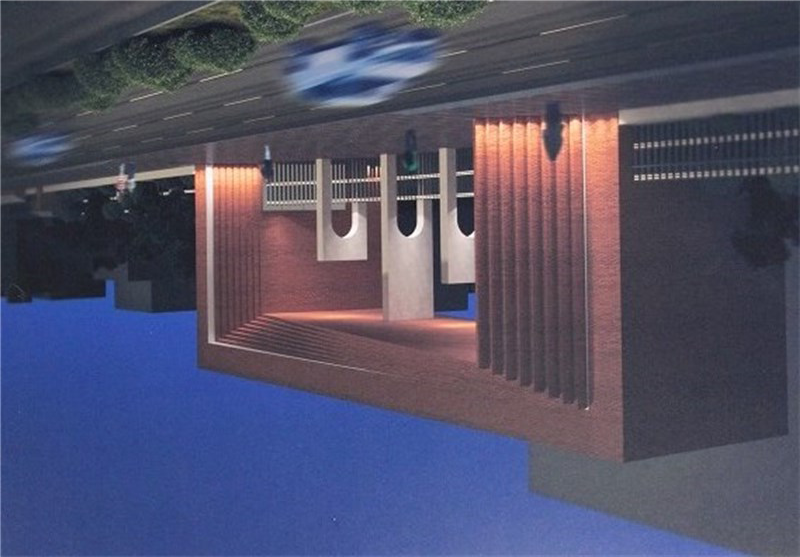
\includegraphics[width=100mm,angle=180]{sharif-door}
    \caption{سر در دانشگاه صنعتی شریف}
    
\end{figure}\\
برای نمایش بهتر سوال ۳ ،ادامه این صفحه را خالی می گذاریم.

\newpage
\subsection*{سوال 3}
ابتدا داده های جدول زیر را بررسی کنید، سپس آنها را تحلیل کرده و نتیجه را بیان نمایید.
\renewcommand{\arraystretch}{1.5}
\begin{table}[h!]
\centering
\begin{tabular}{|l|c|r|} 
 \hline
 انتخاب تیم طراحان&2ماه & 431/651/896 ریال \\
 \hline
 سنجش زاویه زمین &8 ماه & 6/781/901 ریال  \\ 
 \hline
 \multirow{2}{*}{بررسی نحوه ورود دانشجویان به دانشگاه}
 &(خواهران) 5 ماه&540/421/212 ریال
\\ \cline{2-3}
&(برادران) 8 ماه & 12/124/156ریال \\
 \hline
 ساخت & هروقت تموم شه & خیلی خیلی ریال\\
 \hline\hline
\textbf{مجموع}& \textbf{نامشخص}&\textbf{چند ده میلیارد ریال}\\
 \hline
\end{tabular}
\caption{هزینه های پیش بینی شده برای سردر جدید}

\end{table}
\subsection*{انتقادات و پیشنهادات}
در رابطه با آیتم های کلاس کارگاه کامپیوتر (از قبیل کیفیت برگزاری کلاس ها و تدریس، طراحی و تصحیح تمرینات و سایر مواردی که به ذهن میرسد )
پیشنهاداتی که از نظر من میتوان مطرح کرد عبارتند از :
\begin{enumerate}
    \item 
    برای بعضی سوالات تئوری سختگیری زیادی میشد.
    \item
    حجم تکالیف بسیار زیاد و زمان بر و همچنین متناسب با آموزش ها نبود.
    \item
    تعامل بین بچه ها و استاد اصلی اگر باشد ، بازدهی کلاس خیلی بیشتر میشود.
    
\end{enumerate}
همچنین مواردی که می توانست در طول ترم بهتر اجرا شوند عبارتند از:
\begin{itemize}
    \item 
    به نظرم بهتر بود کلاس به جای یک جلسه 3 ساعته در هفته، در دو جلسه 5.1ساعته برگزار میشد.
    \item
    زمان بیشتری برای درس های سخت تر گذاشته شود.
    \item
    آموزش ها پروژه محور شوند (برای مثال استاد تمرین عملی تمر
    ین های پارسال را انجام دهد).\end{itemize}

\end{document}